\chapter{GIS.lab}
\label{2-teorie}

\begin{figure}[H] \centering
    
\includegraphics[width=100pt]{./pictures/gislab-logo.png}
    \caption[GIS.lab logo]{GIS.lab logo (zdroj:
	\href{https://gislab.readthedocs.io/en/latest/_images/gislab-schema.png}{GIS.lab documentation})}
	\label{fig:gislab-logo}
\end{figure}
% zdroj: http://geo.fsv.cvut.cz/~landa/publications/2016/telc-2016/prezentace/figures/

\section{Co je to GIS.lab?}
% https://gislab.readthedocs.io/en/latest/general/about.html
% http://geo.fsv.cvut.cz/~landa/publications/2016/telc-2016/prezentace/landa-telc-2016.pdf
% http://gislab-npo.github.io/gislab/index.html

GIS.lab je nástroj pro jednoduché a rychlé nasazení (deployment) funkční, centrálně spravované \zk{GIS} infrastruktury v jednotném prostředí lokální sítě (\zk{LAN}), data centra nebo cloudové služby. Jedná se o technologii, která poskytuje komplexní soubor otevřených gisových softwarových nástrojů integrovaných do jednoho uživatelsky přívětivého systému, jenž vyžaduje minimální údržbu.

\begin{figure}[H] \centering
    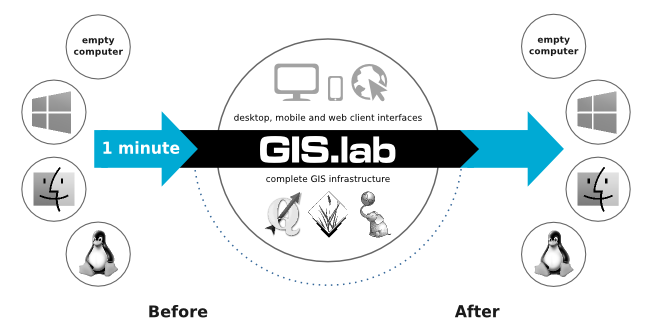
\includegraphics[width=450pt]{./pictures/gislab-schema.png}
    \caption[Schéma jednoduchosti nasazení GIS.lab]{Schéma jednoduchosti nasazení GIS.lab (zdroj:
	\href{https://gislab.readthedocs.io/en/latest/_images/gislab-schema.png}{GIS.lab documentation})}
	\label{fig:gislab-schema}
\end{figure}

Desktopový klient GIS.lab může být ?spuštěn? v režimu fyzickém či virtuálním. Virtuální režim lze využít na kterémkoliv operačním systému (\zk{OS}) s tím, že původní \zk{OS} i GIS.lab jsou přístupné. Fyzický režim umožňuje lepší výkon, který je vykoupen dočasnou nedostupností původního \zk{OS}.

\begin{figure}[H] \centering
    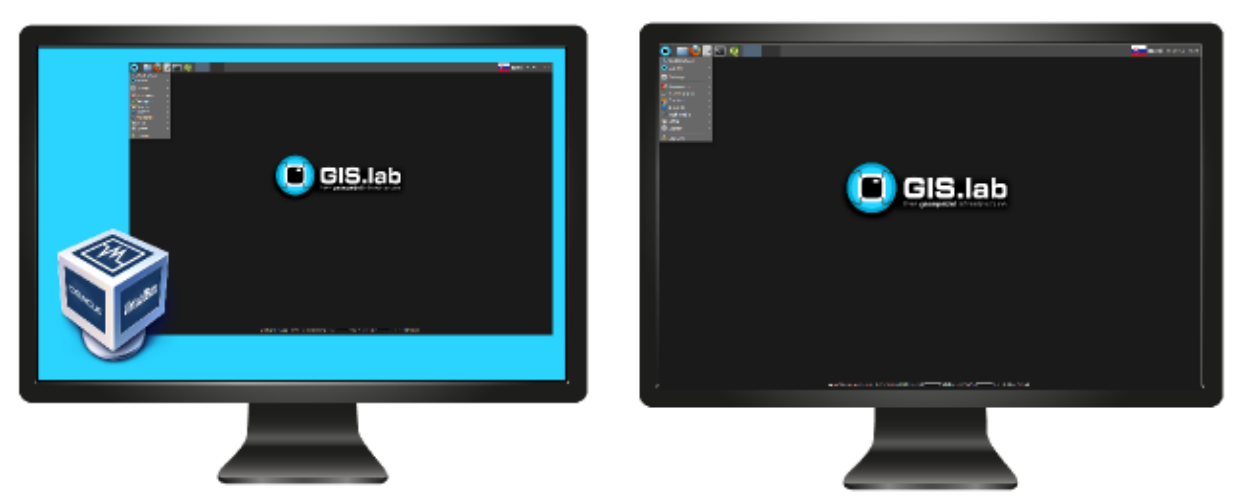
\includegraphics[width=450pt]{./pictures/physical-or-virtual-mode.png}
    \caption[Virtuální a fyzický režim GIS.lab Desktop]{Virtuální a fyzický režim GIS.lab Desktop (zdroj:
	\href{https://gislab.readthedocs.io/en/latest/_images/physical-or-virtual-mode.png}{GIS.lab documentation})}
	\label{fig:gislab-rezim}
\end{figure}

S pomocí integrované platformy Gisquick podporuje GIS.lab kromě desktopového i webového a mobilního klienta. 

\section{Gisquick}
% http://gisquick.org

\begin{figure}[H] \centering
    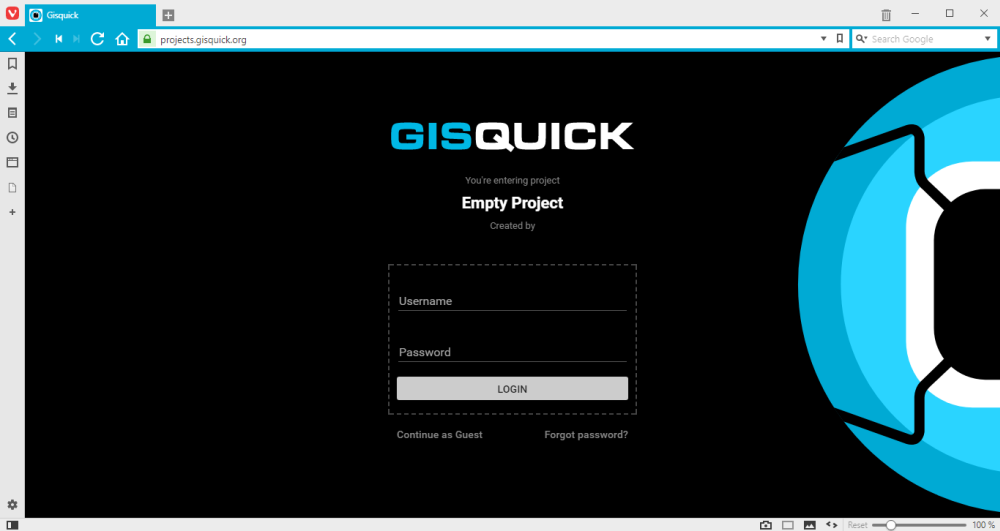
\includegraphics[width=400pt]{./pictures/gisquick-welcome-screen.png}
    \caption[Gisquick - přihlašovací stránka]{Gisquick - přihlašovací stránka (zdroj:
	\href{}{Tereza Kulovaná})}
    \label{fig:gisquick-welcome}
\end{figure}

Gisquick je open-source platforma umožňující publikaci geoprostorových dat. Byla vytvořena s cílem snadného sdílení projektů vytvořených v desktopové aplikaci QGIS na webu. Gisquick sestává ze zásuvného modulu QGIS, QGIS serveru, serverové aplikace založené na frameworku Django, webového a mobilního klientovi. Obsahuje základní sadu nástrojů potřebných pro webovou mapovou aplikaci. Plně responzivní uživatelské rozhraní (\zk{UI}) je optimalizováno i pro mobilní zařízení.

Gisquick byl vyvíjen jako součást GIS.labu, ale v roce xxx se oddělil jako samostatný projekt pod hlavičkou GIS.lab Non-Profit Organization???. Dnes je tedy možné ho využívat samostatně, zároveň však zůstává integrován v každé instalaci GIS.labu a rozšiřuje jeho funkcionalitu.

Je distribuován pod otevřenou licencí GNU \zk{GPL} v2.0.

\section{VISION}
poskytování dalších služeb (kromě tlustého klienta i úložiště dat, sdílení dat, publikace WMS, WFS služeb, publikace přes GisQuick